% cloned from TeXample.net
% modified by Truong Nhan Nguyen

\documentclass[tikz, border=10pt]{standalone}

\usepackage{tikz}
\usetikzlibrary{calc, shapes, positioning}
\usepackage{amsmath, amsfonts, amssymb, mathtools}
\usepackage{mathpazo}

\tikzset{
    club box/.style = {rectangle, rounded corners, draw=red, thick, fill=blue!20, inner sep=10pt, inner ysep=20pt},
    club box title/.style = {rectangle, rounded corners, fill=red, text=white},
    heart box/.style = {rectangle, sharp corners, draw=cyan, thick, fill=green!50, inner sep=10pt, inner ysep=20pt},
    heart box title/.style = {ellipse, fill=cyan!50!black, text=white}
}

\begin{document}
    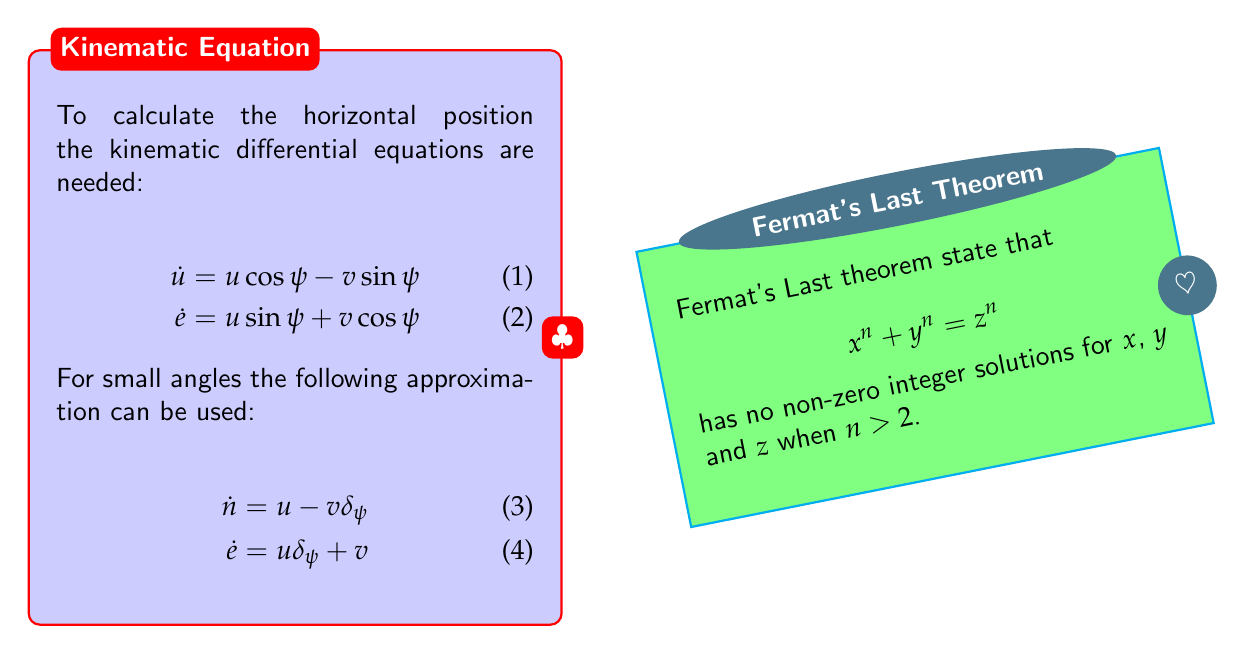
\begin{tikzpicture}
        \node[club box] (cbox) {
            \begin{minipage}{0.5\textwidth}
                \sffamily
                To calculate the horizontal position the kinematic differential equations are needed:\\
                    \begin{align}
                        \dot{u}=u\cos{\psi}-v\sin{\psi}\\
                        \dot{e}=u\sin{\psi}+v\cos{\psi}
                    \end{align}
                For small angles the following approximation can be used:\\
                    \begin{align}
                        \dot{n}=u-v\delta_{\psi}\\
                        \dot{e}=u\delta_{\psi}+v
                    \end{align}
            \end{minipage}
        };
        \node[club box title] (cboxtitle) at ([xshift=2cm]cbox.north west) {\sffamily\bfseries Kinematic Equation};
        \node[club box title] (cboxeasttitle) at (cbox.east) {$\clubsuit$};
        
        \begin{scope}[xshift=8cm, transform shape, baseline, rotate=11.25]
            \node[heart box] (hbox) {
                \sffamily
                \begin{minipage}[t!]{0.5\linewidth}
                    Fermat's Last theorem state that\\
                        \begin{equation*}
                            x^n+y^n=z^n
                        \end{equation*}
                    has no non-zero integer solutions for $x$, $y$ and $z$ when $n>2$.
                \end{minipage}
            };
            \node[heart box title] (hboxtitle) at (hbox.north) {\sffamily\bfseries Fermat's Last Theorem};
            \node[heart box title] (hboxeasttitle) at (hbox.east) {$\heartsuit$};
        \end{scope}
    \end{tikzpicture}
\end{document}